
\documentclass[12pt]{article}
\usepackage{fullpage,amsmath,amssymb,graphicx}

\usepackage{setspace}
\spacing{1}

\usepackage{textpos}
\usepackage{tikz}
\usepackage{pgf}
\usepackage{amssymb}
\usepackage{enumerate}
\usepackage{xcolor}
\usepackage{graphicx}
\usepackage{subcaption}
\usepackage{tabularx}
\usepackage{colortbl}
\usepackage{multicol}
\usepackage{longtable}
\usepackage{hyperref}
\usepackage{comment}
\usepackage{listings}



\definecolor{encabezado}{rgb}{0.74, 0.83, 0.9}

\begin{document}

\hfill\\
\rule{\textwidth}{1.5pt}

\begin{minipage}[t]{85mm}
  \begin{tabular}{l}
    \textbf{\large Instituto Tecnológico de Costa Rica} \\  
    \textbf{Escuela de Ingeniería Electrónica} \\
    \textbf{Trabajo Final de Graduación} \\
    \textbf{Proyecto:} Método basado en aprendizaje reforzado \\para el control automático de una planta no lineal. \\
    \textbf{Estudiante:} Oscar Andrés Rojas Fonseca \hspace{3cm}\rule{4.5cm}{1.5pt}\\
    I Semestre 2024 \hspace{8.5cm}\textbf{Firma del asesor}
  \end{tabular}
\end{minipage}
\hfill\\
\rule{\textwidth}{1.5pt}


\section*{Bitácora de trabajo}

%\begin{table}[h]
\begin{minipage}[h]{\textwidth}
	\centering
	\begin{tabularx}{\textwidth}{|p{2cm}|X|X|p{2cm}|} 
		\hline
		\rowcolor{encabezado}
		\textbf{Fecha} & 
		\textbf{Actividad} & 
		\textbf{Anotaciones} & 
		\textbf{Horas dedicadas} \\ \hline
		% ***************************************************************
	 	24/04/2024 & 
	 	$\mathbf{1}.$ Reunión de seguimiento con el asesor del proyecto. & 
	 	$a)$ Revisión de avance y errores de forma. \newline
	 	$b)$ Se acordó contienuar con el desarrollo de los métodos ajustados para el $PAHM$. \newline & 
	 	2 horas \\
		% ***************************************************************
		26/04/2024 & 
	 	$\mathbf{2}.$ Pruebas de mejora en la función $get\_action()$ del método $PPO$. &
	 	$a)$ Se discute con el asesor respecto al método de exploración y explotación del código base $PPO$. \newline
	 	$b)$ Se decide plantear un cambio escalado del valor inicial de la matriz de covarianza $self.cov\_mat$. \newline
	 	$c)$ Montaje de lógica para cambio de varianza y pruebas con diferentes variación de la desviación estandar. \newline & 
	 	8 horas \\
	 	% ***************************************************************
	 	27/04/2024 & 
	 	$\mathbf{3}.$ Prueba del montaje del método $DQN$ discretizado para el control del env $PAHM$. &
	 	$a)$ Adaptación del código probado con $Pendulum$ al $PAHM$. Ajuste para utilización de la libreria \textit{argparse}. \newline
	 	$b)$ Pruebas de entrenamiento del modelo fallidas por problemas en la función $optimize\_ model()$. \newline & 
	 	6 horas \\
		% ***************************************************************

	 	\hline
	\end{tabularx}
\end{minipage}	 	
	 	
	 	% ***************************************************************
\hfill\\
\begin{minipage}[h]{\textwidth}
	\centering
	\begin{tabularx}{\textwidth}{|p{2cm}|X|X|p{2cm}|} 
		\hline		
		
	 	% ***************************************************************
	 	27/04/2024 & 
	 	$\mathbf{4}.$ Adaptación del código de los métodos para observar los resultados de los entrenamientos mediante la herramienta \textit{Weights $\&$ Biases} (W$\&$B). &
	 	$a)$ Se estudió la forma de enviar la información a W$\&$B. \newline
	 	$b)$ Ajuste de forma para mantener el registro por fecha y hora. \newline & 
	 	4 horas \\
	 	% ***************************************************************
	 	28/04/2024 & 
	 	$\mathbf{5}.$ Continuación de pruebas de variación de varianza y división estandar para el $PPO$ del $PAHM$. &
	 	$a)$ Se crean nuevas versiones de $get\_ action()$ y $evaluate()$ con uso diferentes de distribución normal. \newline
	 	$b)$ Entrenamientos para cada caso de variación. Resultados fallidos. \newline & 
	 	6 horas \\
	 	% ***************************************************************
	 	29/04/2024 & 
	 	$\mathbf{6}.$ Pruebas de entrenamiento del modelo $PPO$ del $PAHM$. &
	 	$a)$ Se probaron diferentes métodos de distribución normal y variaciones de varianza para la etapa de exploración en el entrenamiento. \newline
	 	$b)$ Entrenamiento de modelos con cada método con aproximadamente $150,000$ \textit{timesteps}. El aprendizaje se estanca luego de unos $100,000$ \textit{timesteps}.  \newline & 
	 	6 horas \\ 
	 	% ***************************************************************
	 	30/04/2024 & 
	 	$\mathbf{7}.$ Continuación de entrenamientos con cambios en el valor de la varianza para el método $PPO$. &
	 	$a)$ Se realizan entrenamientos con \textit{timesteps} cercanos a los $500,000$. \newline
	 	$b)$ Algunos resultados presentan cualidades prometedoras, pero en su mayoría no son aceptables. \newline & 
	 	6 horas \\
	 	% ***************************************************************
	 	
	 	\hline
		\multicolumn{3}{|r|}{Total de horas de trabajo:} & 38 horas \\ 
	 	\hline                 
	\end{tabularx}
\end{minipage}





% *****************************************************************************
% *****************************************************************************
% *****************************************************************************

\newpage
\section*{Contenidos de actividades}

Los resultados de los entrenamientos del modelo $PPO$ y sus métodos se compararon con una nueva referencia \href{https://github.com/henanmemeda/RL-Adventure-2/tree/master}{$RL-Adventure-2$} y una anteriormente mencionada como \cite{PPOimplementation}.

Con la implementación de W$\&$B en el código, ahora es posible acceder a los resultados de las pruebas para cada caso del variación con su respectiva fecha y hora, además de ciertos comentarios adicionados en alguna ocación. 

Se cuenta con un proyecto para las pruebas del $PPO$ como se observan en la Figura \ref{fig:wandbPPO} y un proyecto para las pruebas con $DQN$ discreto en la Figura \ref{fig:wandbDQN}.

\begin{figure}[h!]
	\centering
	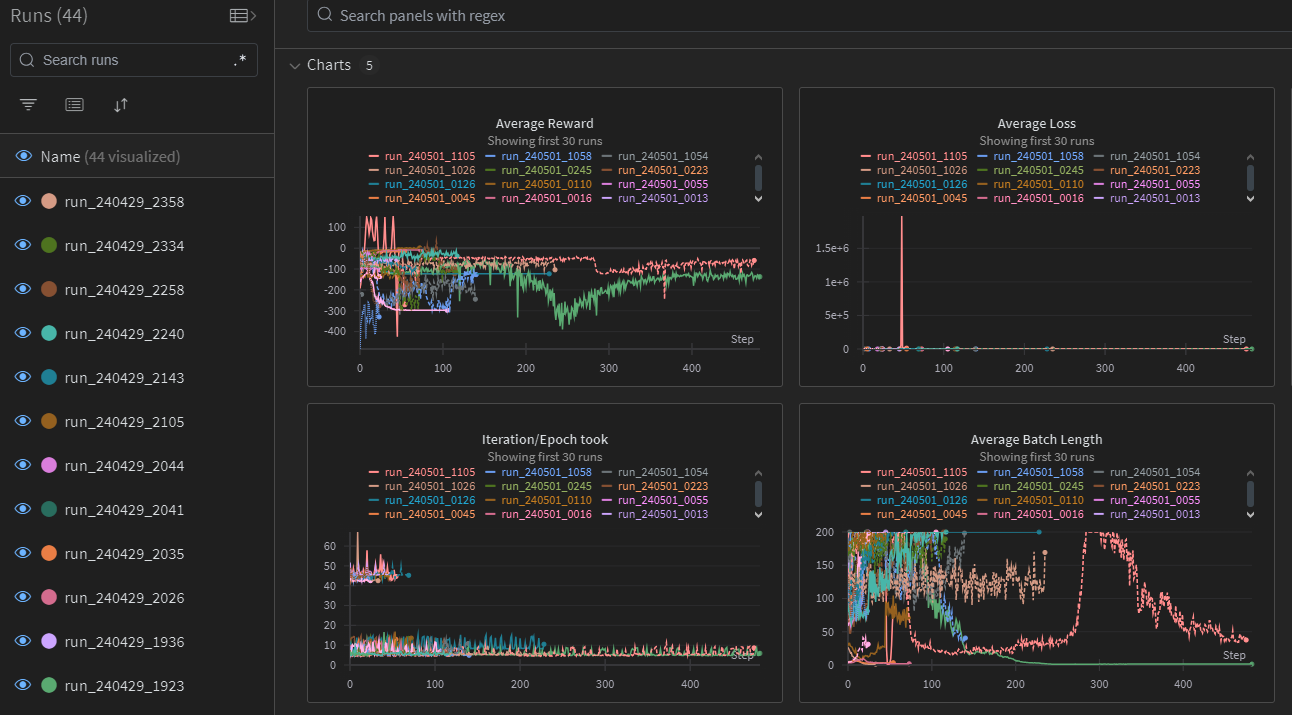
\includegraphics[scale=0.4]{Fig/Captura_wandbPPO.png}
	\caption{Pruebas de entrenamiento del modelo $PahmPPO$ en $wandb$.}
	\label{fig:wandbPPO}
\end{figure}	

\begin{figure}[h!]
	\centering
	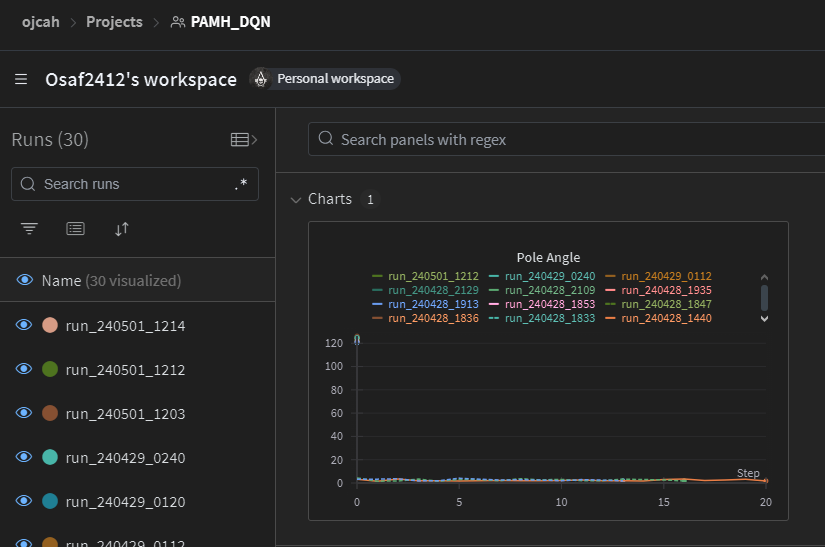
\includegraphics[scale=0.45]{Fig/Captura_wandbDQN.png}
	\caption{Pruebas de entrenamiento del modelo $PahmDQN$ en $wandb$.}
	\label{fig:wandbDQN}
\end{figure}	


\newpage

\section*{Referencias}
\renewcommand\refname{}
\bibliographystyle{IEEEtran}
\bibliography{references}





\end{document}
